\section{Análisis de interrelaciones}

   \paragraph{}Una vez definidas las distintas entidades presentes en el
   modelo, a continuación se detallarán las distintas relaciones que mantienen
   entre ellas. Las interrelaciones por describir son las siguientes:

   \begin{itemize}
    \item Interrelación Administrador Centro - Centro.
    \item Interrelación Centro - Titulación.
    \item Interrelación Titulación - Asignatura.
    \item Interrelación Asignatura - Asignatura Curso Académico.
    \item Interrelación Asignatura Curso Académico - Alumno Curso Académico.
    \item Interrelación Alumno - Alumno Curso Académico.
    \item Interrelación Asesor - Alumno Curso Académico.
    \item Interrelación Departamento - Asesor Curso Académico.
   \end{itemize}

   \paragraph{}Para la descripción de cada relación entre entidades, se
   utilizarán los siguientes apartados:

   \begin{description}
      \item[Definición] Especifica el motivo por el cual se produce la
           interrelación y entre qué tipos de entidad se da lugar.

      \item[Características] En este aparatado se mostrará la siguiente
           información:

            \begin{itemize}
             \item Nombre del tipo de interrelación.
             \item Tipo de la interrelación, es decir, fuerte o débil. En el
                   caso de que sea débil se especifica el tipo de debilidad:
                   existencia o identificación.
             \item Cardinalidad de la interrelación y cardinalidad con la que
                   cada tipo de entidad participa en la interrelación.
             \item Número de atributos del tipo de interrelación.
            \end{itemize}

      \item[Diagrama] Representación gráfica del tipo de interrelación.

      \item[Descripción de los atributos] Se describirán cada uno de los
           atributos que forman parte del tipo de interrelación. Para cada uno
           de ellos se indicará lo siguiente:

           \begin{itemize}
            \item Definición del atributo.
            \item Dominio en el cual se encuentra.
            \item Ejemplo práctico de cada atributo.
           \end{itemize}

      \item[Ejemplo práctico del tipo de interrelación] En este apartado se
           muestra una ocurrencia concreta del tipo de interrelación.
   \end{description}

\subsection{Interrelación Administrador Centro - Centro}

   \begin{description}
      \item[Definición] En esta interrelación se deja constancia de que cada
      centro establecido en el sistema dispone, al menos, un administrador de
      centro.

      \item[Características] La interrelación presenta las siguientes
                             características:

         \begin{itemize}
            \item \textbf{Nombre:} AC-C
            \item \textbf{Tipo de la interrelación:} Fuerte
            \item \textbf{Cardinalidad de la interrelación:} N:M
                  \begin{itemize}
                     \item Administrador Centro: administra (0,n)
                     \item Centro: es\_administrado\_por (1,n)
                  \end{itemize}
            \item \textbf{Número de atributos:} Ninguno
         \end{itemize}

      \item[Diagrama] La figura \ref{diagramaAC-C} muestra el diagrama de la
                      interrelación.
      \item \begin{figure}[!ht]
            \begin{center}
            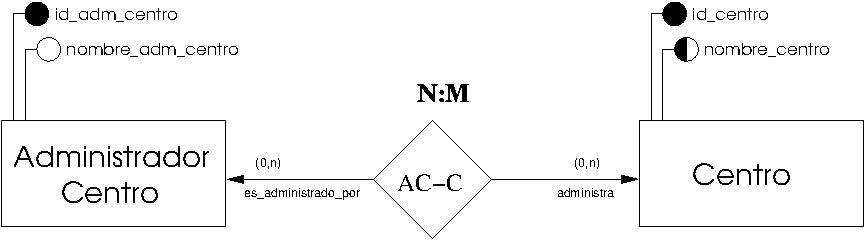
\includegraphics[]{07.Modelo_Entidad-Interrelacion/7.3.Analisis_Interrelaciones/diagramas/AC-C.pdf}
            \caption{Diagrama de la interrelación AC-C.}
            \label{diagramaAC-C}
            \end{center}
         \end{figure}

      \item[Ejemplo práctico del tipo de interrelación]

      \item \begin{center}
            \begin{tabular}{ | c | c | }
            \hline
            \multicolumn{2}{ | c | }{\textbf{Tipo de interrelación AC-C}} \\
            \hline
            \textbf{Administrador Centro} & \textbf{Centro}\\
            \hline
            id\_adm\_centro & id\_centro \\
            \hline
            9 & 15 \\
            \hline
            \end{tabular}
         \end{center}

   \end{description}

\subsection{Interrelación Centro - Titulación}

   \begin{description}
      \item[Definición]

      \item[Características] La interrelación presenta las siguientes
                             características:

         \begin{itemize}
            \item \textbf{Nombre:}
            \item \textbf{Tipo de la interrelación:}
            \item \textbf{Cardinalidad de la interrelación:}
            \item \textbf{Número de atributos:}
         \end{itemize}

      \item[Diagrama] La figura \textit{RELLENAR} muestra el diagrama de la
                      interrelación.

      \item[Descripción de los atributos]

      \item[Ejemplo práctico del tipo de interrelación]
   \end{description}

\subsection{Interrelación Titulación - Asignatura}

   \begin{description}
      \item[Definición] En esta interrelación se deja constancia de que cada
      titulación establecida en el sistema podrá disponer de varias asignaturas.

      \begin{itemize}
       \item Una titulación puede disponer de varias asignaturas.
       \item Una asignatura solamente puede pertenecer a una determinada
             titulación.
      \end{itemize}

      \item[Características] La interrelación presenta las siguientes
                             características:

         \begin{itemize}
            \item \textbf{Nombre:} T-A
            \item \textbf{Tipo de la interrelación:} El tipo de entidad
                  Asignatura es débil por identificación respecto al tipo de
                  entidad Titulación.
            \item \textbf{Cardinalidad de la interrelación:} 1:N
                  \begin{itemize}
                     \item Titulación: dispone\_de (0,n)
                     \item Asignatura: pertenece\_a (1,1)
                  \end{itemize}
            \item \textbf{Número de atributos:} Ninguno.
         \end{itemize}

      \item[Diagrama] La figura \ref{diagramaT-A} muestra el diagrama de la
                      interrelación.

      \item \begin{figure}[!ht]
            \begin{center}
            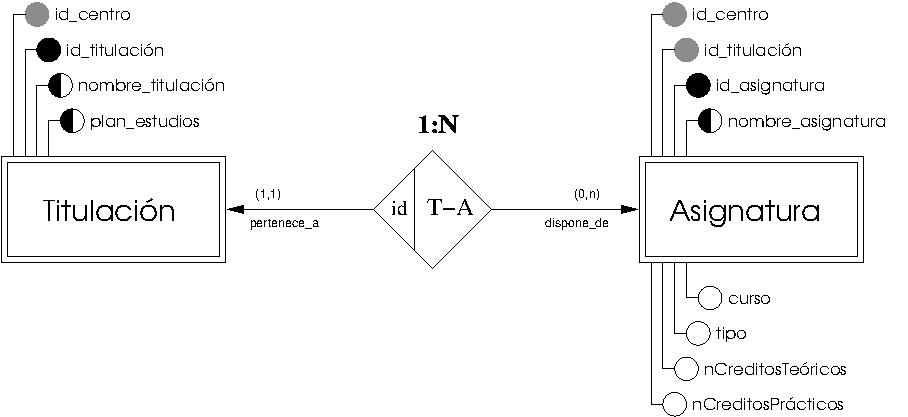
\includegraphics[]{07.Modelo_Entidad-Interrelacion/7.3.Analisis_Interrelaciones/diagramas/T-A.pdf}
            \caption{Diagrama de la interrelación T-A.}
            \label{diagramaT-A}
            \end{center}
         \end{figure}

      \item[Ejemplo práctico del tipo de interrelación]

      \item \begin{center}
            \begin{tabular}{ | r r | }
            \hline
            \multicolumn{2}{ | c | }{\textbf{Tipo de interrelación T-A}} \\
            \hline
            \textbf{Titulación} & \\
            id\_centro & 15 \\
            id\_titulación & 3 \\
            \hline
            \textbf{Asignatura} & \\
            id\_centro & 15 \\
            id\_titulación & 3 \\
            id\_asignatura & 17 \\
            \hline
            \end{tabular}
         \end{center}
   \end{description}

\subsection{Interrelación Asignatura - Asignatura Curso Académico}

   \begin{description}
      \item[Definición]

      \item[Características] La interrelación presenta las siguientes
                             características:

         \begin{itemize}
            \item \textbf{Nombre:}
            \item \textbf{Tipo de la interrelación:}
            \item \textbf{Cardinalidad de la interrelación:}
            \item \textbf{Número de atributos:}
         \end{itemize}

      \item[Diagrama] La figura \textit{RELLENAR} muestra el diagrama de la
                      interrelación.

      \item[Descripción de los atributos]

      \item[Ejemplo práctico del tipo de interrelación]
   \end{description}

\subsection{Interrelación Asignatura Curso Académico - Alumno Curso Académico}

   \begin{description}
      \item[Definición] En esta interrelación se deja constancia de que un
      alumno matriculado durante un curso académico está matriculado de un
      determinado de un número indeterminado de asignaturas, las cuales
      pertenecen a un determinado curso académico.

      \item[Características] La interrelación presenta las siguientes
                             características:

         \begin{itemize}
            \item \textbf{Nombre:} ACA-AlCA
            \item \textbf{Tipo de la interrelación:} Fuerte.
            \item \textbf{Cardinalidad de la interrelación:} N:M
            \item \textbf{Número de atributos:} 1, nota.
         \end{itemize}

      \item[Diagrama] La figura \ref{diagramaACA-AlCA} muestra el diagrama de la
                      interrelación.

       \item \begin{figure}[!ht]
            \begin{center}
            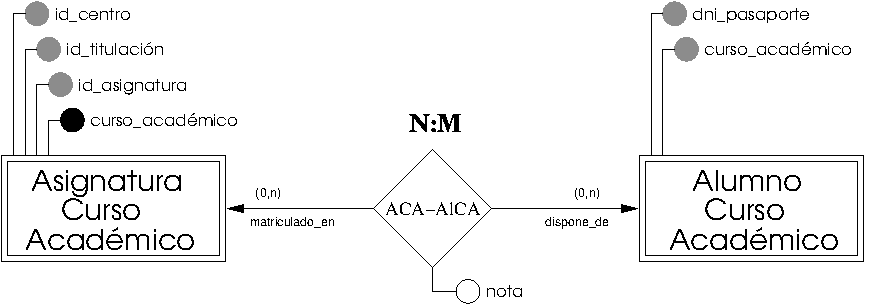
\includegraphics[]{07.Modelo_Entidad-Interrelacion/7.3.Analisis_Interrelaciones/diagramas/ACA-AlCA.pdf}
            \caption{Diagrama de la interrelación ACA-AlCA.}
            \label{diagramaACA-AlCA}
            \end{center}
         \end{figure}

      \item[Descripción de los atributos]

      \item \begin{description}
               \item[Nota] Establece la calificación obtenida por un alumno en
               una asignatura durante un curso académico.
             \end{description}

      \item[Ejemplo práctico del tipo de interrelación]

      \item \begin{center}
            \begin{tabular}{ | r r | }
            \hline
            \multicolumn{2}{ | c | }{\textbf{Tipo de interrelación ACA-AlCA}} \\
            \hline
            \textbf{Asignatura Curso Académico} & \\
            id\_centro & 15 \\
            id\_titulación & 3 \\
            id\_asignatura & 17 \\
            curso\_académico & 2008\\
            \hline
            \textbf{Alumno Curso Académico} & \\
            dni\_pasaporte & 01234567A \\
            curso\_académico & 2008 \\
            \hline
            \textbf{Atributos} & \\
            nota & 7,5 \\
            \hline
            \end{tabular}
         \end{center}
   \end{description}

\subsection{Interrelación Alumno - Alumno Curso Académico}

   \begin{description}
      \item[Definición] En esta interrelación se deja constancia de que un
      alumno puede estar matriculado durante un número indeterminado de cursos
      académicos.

      \item[Características] La interrelación presenta las siguientes
                             características:

         \begin{itemize}
            \item \textbf{Nombre:} A-AlCA
            \item \textbf{Tipo de la interrelación:} El tipo de entidad
                  Alumno Curso Académico es débil por identificación respecto al
                  tipo de entidad Alumno.
            \item \textbf{Cardinalidad de la interrelación:} 1:N
                  \begin{itemize}
                     \item Alumno: matriculado\_en (0,n)
                     \item Alumno Curso Académico: es\_un (1,1)
                  \end{itemize}
            \item \textbf{Número de atributos:} Ninguno.
         \end{itemize}

      \item[Diagrama] La figura \ref{diagramaA-AlCA} muestra el diagrama de la
                      interrelación.

      \item \begin{figure}[!ht]
            \begin{center}
            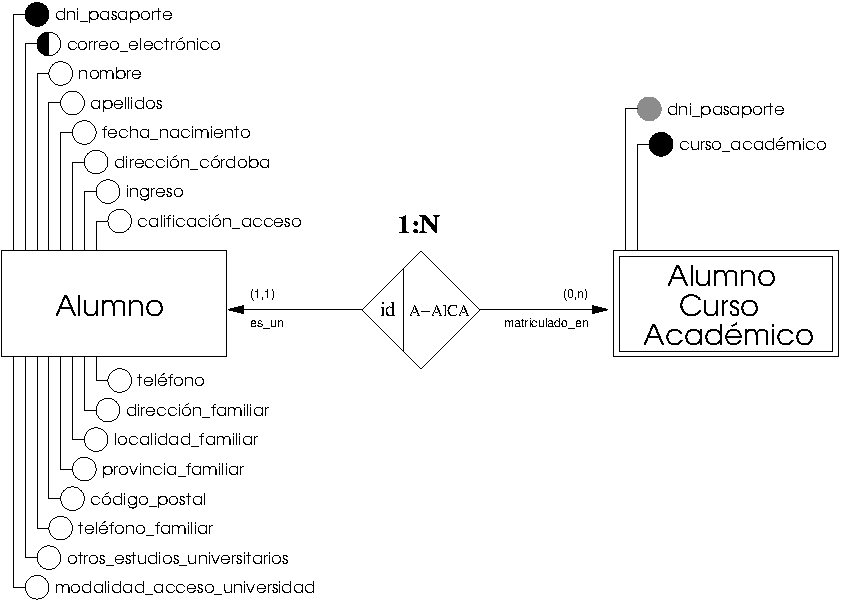
\includegraphics[]{07.Modelo_Entidad-Interrelacion/7.3.Analisis_Interrelaciones/diagramas/A-AlCA.pdf}
            \caption{Diagrama de la interrelación A-AlCA.}
            \label{diagramaA-AlCA}
            \end{center}
         \end{figure}

      \item[Ejemplo práctico del tipo de interrelación]

      \item \begin{center}
            \begin{tabular}{ | r r | }
            \hline
            \multicolumn{2}{ | c | }{\textbf{Tipo de interrelación A-AlCA}} \\
            \hline
            \textbf{Alumno} & \\
            dni\_pasaporte & 01234567A \\
            \hline
            \textbf{Alumno Curso Académico} & \\
            dni\_pasaporte & 01234567A \\
            curso\_académico & 2008 \\
            \hline
            \end{tabular}
         \end{center}
   \end{description}

\subsection{Interrelación Asesor - Alumno Curso Académico}

   \begin{description}
      \item[Definición] En esta interrelación se deja constancia de que un
      asesor puede ofrecer servicios de asesoría a un número indeterminado
      de alumnos matriculados durante un determinado curso académico.

      \item[Características] La interrelación presenta las siguientes
                             características:

         \begin{itemize}
            \item \textbf{Nombre:} As-AlCA
            \item \textbf{Tipo de la interrelación:} El tipo de entidad
                  Alumno Curso Académico es débil por existencia respecto al
                  tipo de entidad Asesor.
            \item \textbf{Cardinalidad de la interrelación:} 1:N
            \item \textbf{Número de atributos:} Ninguno.
         \end{itemize}

      \item[Diagrama] La figura \ref{diagramaAs-AlCA} muestra el diagrama de la
                      interrelación.

      \item \begin{figure}[!ht]
            \begin{center}
            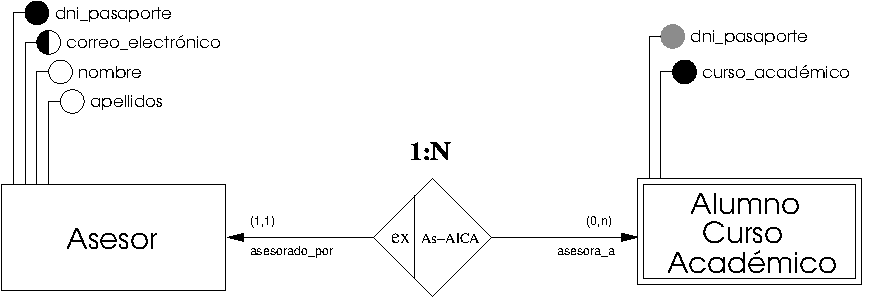
\includegraphics[]{07.Modelo_Entidad-Interrelacion/7.3.Analisis_Interrelaciones/diagramas/As-AlCA.pdf}
            \caption{Diagrama de la interrelación As-AlCA.}
            \label{diagramaAs-AlCA}
            \end{center}
         \end{figure}

      \item[Ejemplo práctico del tipo de interrelación]

      \item \begin{center}
            \begin{tabular}{ | r r | }
            \hline
            \multicolumn{2}{ | c | }{\textbf{Tipo de interrelación As-AlCA}} \\
            \hline
            \textbf{Asesor} & \\
            dni\_pasaporte & 98765432Z \\
            \hline
            \textbf{Alumno Curso Académico} & \\
            dni\_pasaporte & 01234567A \\
            id\_centro & 2008 \\
            \hline
            \end{tabular}
         \end{center}
   \end{description}

\subsection{Interrelación Departamento - Asesor Curso Académico}

   \begin{description}
      \item[Definición] En esta interrelación se deja constancia de que un
      asesor puede ofrecer servicios de asesoría perteneciendo a un departamento
      durante un determinado curso académico.

      \item[Características] La interrelación presenta las siguientes
                             características:

         \begin{itemize}
            \item \textbf{Nombre:} D-AseCA
            \item \textbf{Tipo de la interrelación:} El tipo de entidad
                  Asesor Curso Académico es débil por existencia respecto al
                  tipo de entidad Departamento.
            \item \textbf{Cardinalidad de la interrelación:} 1:N
            \item \textbf{Número de atributos:} Ninguno.
         \end{itemize}

      \item[Diagrama] La figura \ref{diagramaD-AseCA} muestra el diagrama de la
                      interrelación.

      \item \begin{figure}[!ht]
            \begin{center}
            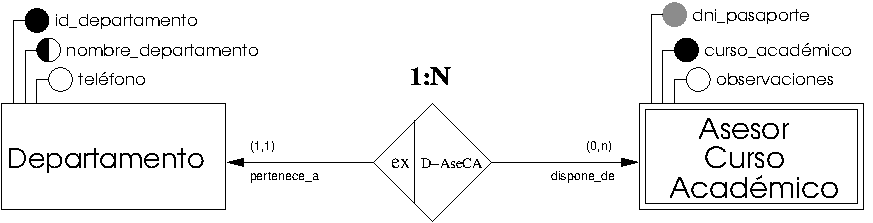
\includegraphics[]{07.Modelo_Entidad-Interrelacion/7.3.Analisis_Interrelaciones/diagramas/D-AseCA.pdf}
            \caption{Diagrama de la interrelación D-AseCA.}
            \label{diagramaD-AseCA}
            \end{center}
         \end{figure}

      \item[Ejemplo práctico del tipo de interrelación]

      \item \begin{center}
            \begin{tabular}{ | r r | }
            \hline
            \multicolumn{2}{ | c | }{\textbf{Tipo de interrelación D-AseCA}} \\
            \hline
            \textbf{Departamento} & \\
            id\_departamento & 22 \\
            \hline
            \textbf{Asesor Curso Académico} & \\
            dni\_pasaporte & 98765432Z \\
            curso\_académico & 2007 \\
            \hline
            \end{tabular}
         \end{center}
   \end{description}

